%%%%%%%%%%%%%%%%%%%%%%%%%%%%%%%%%%%%%%%%%%%%%%%%%%%%%%%%%%%%%%%%%%%%%%%%%%%%%%%%

\begin{frame}{Implementation Strategy}

\begin{itemize}
    \item Create test kernels
    \begin{itemize}
        \item Start with very simple kernels (e.g. copy buffer, add two buffers)
        \item Gradually add more features (e.g. non-sequential memory accesses, vector instructions, etc)
    \end{itemize}
    
    \item Suggested implementation order
    \begin{itemize}
        \item Preparation and packetization first (required for simplest kernels)
        \item Then easier features: builtins, memory addressing, scalarization, instantiation
        \item More complex features last: control flow, optimizations
    \end{itemize}
\end{itemize}

\end{frame}

%%%%%%%%%%%%%%%%%%%%%%%%%%%%%%%%%%%%%%%%%%%%%%%%%%%%%%%%%%%%%%%%%%%%%%%%%%%%%%%%

\begin{frame}{Scalarization Process}

\begin{itemize}
    \item Look for vector \varying{varying} instructions such as:
    \begin{itemize}
        \item Leaves that define vector values, vector stores
        \item Vector extractions
        \item Vector -> scalar bitcasts
    \end{itemize}
    
    \item Recursively scalarize until we reach a scalar value
    \begin{itemize}
        \item Operands before instructions
        \item Re-create instructions for each vector element
        \item Vector lane $\neq$ SIMD instance!
    \end{itemize}
    
\end{itemize}

\end{frame}

%%%%%%%%%%%%%%%%%%%%%%%%%%%%%%%%%%%%%%%%%%%%%%%%%%%%%%%%%%%%%%%%%%%%%%%%%%%%%%%%

%\begin{frame}[c]{Scalarization Example: Before}
%
%\center{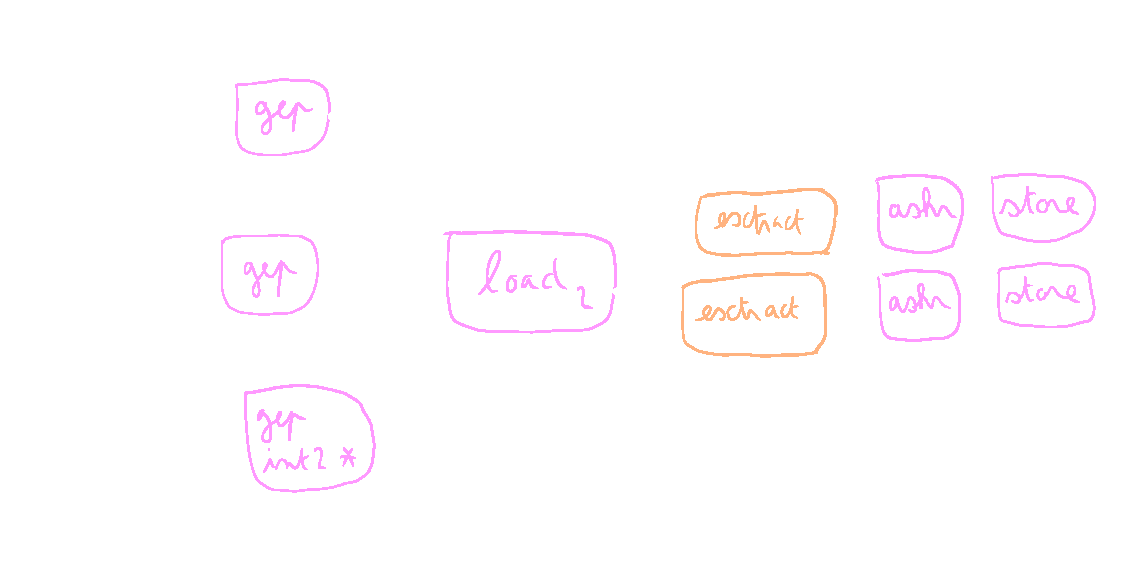
\includegraphics[scale=0.65]{images/scalarization-start.pdf}}
%
%\end{frame}

%%%%%%%%%%%%%%%%%%%%%%%%%%%%%%%%%%%%%%%%%%%%%%%%%%%%%%%%%%%%%%%%%%%%%%%%%%%%%%%%

%\begin{frame}{Scalarization Example: After}
%
%\center{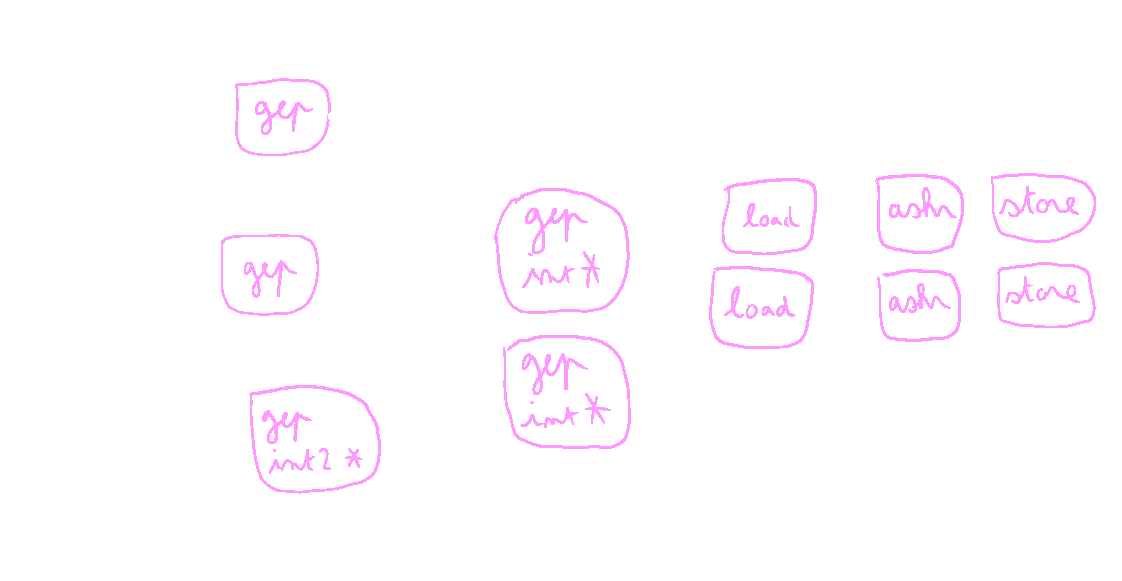
\includegraphics[scale=0.65]{images/scalarization-end.pdf}}
%
%\end{frame}

%%%%%%%%%%%%%%%%%%%%%%%%%%%%%%%%%%%%%%%%%%%%%%%%%%%%%%%%%%%%%%%%%%%%%%%%%%%%%%%%

\begin{frame}[fragile]{Scalarization Example}

After Scalarization:
\begin{codebox}
kernel void extract_lr(int2 *src, int *left, int *right) {
    int tid = get_global_id(0);
    int sampleLeft = *((int *)&src[tid] + 0);
    int sampleRight = *((int *)&src[tid] + 1);
    left[tid] = (sampleLeft >> 1);
    right[tid] = (sampleRight >> 1);
}
\end{codebox}

After Packetization:
\begin{codebox}
kernel void extract_lr(int2 *src, int *left, int *right) {
    int tid = get_global_id(0);
    int4 samplesLeft  = interleaved_load_int4((int *)&src[tid] + 0, 2);
    int4 samplesRight = interleaved_load_int4((int *)&src[tid] + 1, 2);
    vstore4(samplesLeft >> 1, tid, (int *)left);
    vstore4(samplesRight >> 1, tid, (int *)right);
}
\end{codebox}

\end{frame}
